% LaTeX source for textbook ``ThinkCPP , a game perspective''
% Copyright (C) 2023  Lisa Patacchiola and Allen B Downey


\chapter{Variables and types}

\section{More output}
\index{output}
\index{statement!output}

As I mentioned in the last chapter, you can put as many statements as
you want in {\tt main}.  For example, to output more than one line:

\begin{lstlisting}[frame=single]
#include <iostream>

// main: generate some simple output

int main ()
{
  // output 1 line
  std::cout << "Hello, world." << std::endl; 
  
  // output 1 more
  std::cout << "How are you?" << std::endl;  
  return 0;
}
\end{lstlisting}

As you can see, it is legal to put comments at the
end of a line, as well as on a line by themselves.

\index{replit}
If you want to try that with the replit code, go back to the project link 
\url{https://replit.com/@lpatacch/helloWorld#hello.cpp}. Then, look for a button on the right hand of the screen with the words "Fork Repl". It should look like Figure \ref{fig:fork}
\begin{figure}
    \centering
    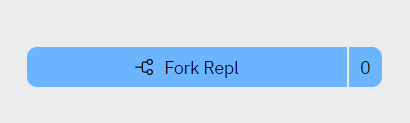
\includegraphics{fork}
    \caption{The Fork button on Replit}
    \label{fig:fork}
\end{figure}
You now should have a copy of the code that you can change any way you want.

\index{string}
\index{type!string}

In the program. the phrases that appear in quotation marks are called {\bf strings},
because they are made up of a sequence (string) of letters.  Actually,
strings can contain any combination of letters, numbers, punctuation
marks, and other special characters.

\index{newline}

Often it is useful to display the output from multiple output
statements all on one line.  You can do this by leaving out
the first {\tt endl}:

\begin{lstlisting}[frame=single]
int main ()
{
  std::cout << "The game ";
  std::cout << "is about to start!" << std::endl;
  return 0
}
\end{lstlisting}

In this case the output appears on a single line as
{\tt The game is about to start!}.  Notice that there is a space
between the word ``game'' and the second quotation mark.
This space appears in the output, so it affects the behavior
of the program.

Spaces that appear outside of quotation marks generally do
not affect the behavior of the program.  For example, I
could have written:

\begin{lstlisting}[frame=single]
int main ()
{
  std::cout<<"The game";
  std::cout<<" is about to start!"<<std::endl;
  return 0;
}
\end{lstlisting}

This program would compile and run just as well as the original.
The breaks at the ends of lines (newlines) do not affect
the program's behavior either, so I could have written:

\begin{lstlisting}[frame=single]
int main(){std::cout<<"The game ";std::cout<<
    "is about to start!"<<std::endl;return 0;}
\end{lstlisting}

That would work, too, although you have probably noticed that
the program is getting harder and harder to read.  Newlines and
spaces are useful for organizing your program visually, making
it easier to read the program and locate syntax errors.

\section{Values}
\index{value}
\index{type}

A value is one of the fundamental things---like a letter or
a number---that a program manipulates.  The only values we have
manipulated so far are the string values we have been outputting, like
{\tt "Hello, world."}.  You (and the compiler) can identify
string values because they are enclosed in quotation marks.

There are other kinds of values, including integers and characters.
An integer is a whole number like 1 or 17.  You can output
integer values the same way you output strings:

\begin{lstlisting}
  std::cout << 17 << std::endl;
\end{lstlisting}

A character value is a letter or digit or punctuation mark
enclosed in single quotes, like {\tt 'a'} or {\tt '5'}.
You can output character values the same way:


\begin{lstlisting}
  std::cout << '}' << std::endl;
\end{lstlisting}

This example outputs a single close squiggly-brace on a line
by itself.

It is easy to confuse different types of values, like {\tt "5"}, {\tt
'5'} and {\tt 5}, but if you pay attention to the punctuation, it
should be clear that the first is a string, the second is a character
and the third is an integer.  The reason this distinction is important
should become clear soon.

\section {Variables}
\index{variable}
\index{value}

One of the most powerful features of a programming language is the
ability to manipulate {\bf variables}.  A variable is a named location
that stores a value.  

Just as there are different types of values (integer, character,
etc.), there are different types of variables.  When you create a new
variable, you have to declare what type it is.  For example, the
character type in C++ is called {\tt char}.  The following statement
creates a new variable named {\tt sarah} that has type {\tt char}.

\begin{lstlisting}
    char sarah;
\end{lstlisting}

This kind of statement is called a {\bf declaration}.

The type of a variable determines what kind of values it can
store.  A {\tt char} variable can contain characters, and it should
come as no surprise that {\tt int} variables can store integers.

There are several types in C++ that can store string values, but we
are going to skip that for now (see Chapter~\ref{strings}).

\index{declaration}
\index{statement!declaration}

To create an integer variable, the syntax is 

\begin{lstlisting}
    int bob;
\end{lstlisting}
%
where {\tt bob} is the arbitrary name you made up for the
variable.  In general, you will want to make up variable names
that indicate what you plan to do with the variable.  For
example, if you saw these variable declarations:

\begin{lstlisting}
    char firstLetter;
    char lastLetter;
    int hour, minute;
\end{lstlisting}
%
you could probably make a good guess at what values
would be stored in them.  This example
also demonstrates the syntax for declaring multiple variables
with the same type: {\tt hour} and {\tt minute}
are both integers ({\tt int} type).

\section{Assignment}
\index{assignment}
\index{statement!assignment}

Now that we have created some variables, we would like to
store values in them.  We do that with an {\bf assignment
statement}.


\begin{lstlisting}
    firstLetter = 'a';   // give firstLetter the 
                         // value 'a'
    hour = 11;           // assign the value 11 to hour
    minute = 59;         // set minute to 59
\end{lstlisting}
%
This example shows three assignments, and the comments show
three different ways people sometimes talk about assignment
statements.  The vocabulary can be confusing here, but the
idea is straightforward:

\begin{itemize}

\item When you declare a variable, you create a named storage location.

\item When you make an assignment to a variable, you give it a value.

\end{itemize}

A common way to represent variables on paper is to draw a box
with the name of the variable on the outside and the value
of the variable on the inside.  This kind of figure is called
a {\bf state diagram} because is shows what state each of the
variables is in (you can think of it as the variable's ``state of
mind'').
This diagram shows
the effect of the three assignment statements:

\vspace{0.1in}
\centerline{\epsfig{figure=assign.eps}}
\vspace{0.1in}

\index{rules!variable value}
I sometimes use different shapes to indicate different
variable types.  These shapes should help remind you that one of the
rules in C++ is that a variable has to have the same type as the
value you assign it.  For example, you cannot store a string in
an {\tt int} variable.  The following statement generates a compiler
error.

\begin{lstlisting}
  int hour;
  hour = "Hello.";       // WRONG !!
\end{lstlisting}

%
This rule is sometimes a source of confusion, because there are many
ways that you can convert values from one type to another, and C++
sometimes converts things automatically.  But for now you should
remember that as a general rule variables and values have the same
type, and we'll talk about special cases later.

Another source of confusion is that some strings {\em look}
like integers, but they are not.  For example,
the string {\tt "123"}, which is made up of the
characters {\tt 1}, {\tt 2} and {\tt 3}, is not
the same thing as the {\em number} {\tt 123}.
This assignment is illegal:

\begin{lstlisting}
  minute = "59";         // WRONG!
\end{lstlisting}
%
\section{Initialization}
When variables are created, they can be set to a value immediately instead of waiting until later. This can shorten your code. 

\subsection{Legacy}
Pre-C++ 11, it was quite common to use an equation to initialize 
your variables.
Here is an example:
\begin{lstlisting}
  int hitPoints = 10;
\end{lstlisting}
Most of our examples use this format, because people are used to 
this style when using other computer languages. But, C++11 and later
have a different style that can be used instead.
\subsection{Braced}
This new style is called braced initialization. Instead of having an equal sign, the line is even shorter. Although it does the same thing as the equal sign, it can help with some common programming errors. We will be talking about this in later chapters.
\begin{lstlisting}
  int hitPoints{10};
\end{lstlisting}
\index{braced initialization}
\index{initalization!braced}
\section{Outputting variables}
\label{output}

You can output the value of a variable using the same commands
we used to output simple values.

\begin{lstlisting}[frame=single]
  int hour, minute;
  char colon;

  hour = 11;
  minute = 59;
  colon = ':';

  std::cout << "The battle will start at  ";
  std::cout << hour;
  std::cout << colon;
  std::cout << minute;
  std::cout << std::endl;
\end{lstlisting}

%
Try this project here:\url{https://replit.com/@lpatacch/OutputVariables#outvar.cpp}.
This program creates two integer variables named {\tt hour} and {\tt
minute}, and a character variable named {\tt colon}.  It assigns
appropriate values to each of the variables and then uses a series
of output statements to generate the following:

\begin{verbatim}
The battle will start at 11:59
\end{verbatim}

When we talk about ``outputting a variable,'' we mean outputting the
{\em value} of the variable.  To output the {\em name} of a variable,
you have to put it in quotes.  For example: {\tt std::cout << "hour";}

As we have seen before, you can include more than one value in
a single output statement, which can make the previous program more
concise:

\begin{lstlisting}[frame=single]
  int hour, minute;
  char colon;

  hour = 11;
  minute = 59;
  colon = ':';

  std::cout << "The battle will start at " << hour 
                << colon << minute << std::endl;
\end{lstlisting}
%
On one line, this program outputs a string, two integers, a character,
and the special value {\tt endl}.  Very impressive!


\section{Variable Naming Rules}
\index{variable naming rules}
\index{variable!naming rules}
\index{rules!variable naming}
A few sections ago, I said that you can make up any name you
want for your variables, but that's not quite true. There are certain rules that you need to follow.
\begin{enumerate}
    \item The name can not start with a number. (It is ok for a number to be in the name, it just can't be the first letter.)
    \item No spaces in the name
    \item Capitalization matters (num is different than NUM) 
    \item No special characters can be in the name other than underscore.
\end{enumerate}

Here are some examples of variables that do not follow the naming rules, and what you can use instead
\begin{lstlisting}[frame=single]
    int 3player;    \\ WRONG, can not start with a 
                    \\ number
    int player3;    \\ This would work
    int my3player   \\ This will also work
    
    int hit points; \\ WRONG, spaces not allowed in the 
                    \\ name
    int hitPoints;  \\ This would work
    int hit_points; \\ This also would work
    
    int cash$;      \\ This would not work because of 
                    \\ $sign
    int cashMoney;  \\ changed to use words instead
\end{lstlisting}
\subsection{Keywords}
\index{keyword}
In addition, there
are certain words that are reserved in C++ because they are
used by the compiler to parse the structure of your program,
and if you use them as variable names, it will get confused.
These words, called {\bf keywords}, include {\tt int},
{\tt char}, {\tt void}, {\tt endl} and many more.

The complete list of keywords is included in the C++ Standard, which
is the official language definition adopted by the the International
Organization for Standardization (ISO) on September 1, 1998.  You
can download a copy electronically from
\bigskip

    \url{http://www.ansi.org/}
%
\bigskip

Rather than memorize the list, I would suggest that you
take advantage of a feature provided in many development
environments: code highlighting.  As you type, different
parts of your program should appear in different colors.  For
example, keywords might be blue, strings red, and other code
black.  If you type a variable name and it turns blue, watch
out!  You might get some strange behavior from the compiler.

\section{Operators}
\index{operator}

{\bf Operators} are special symbols that are used to represent
simple computations like addition and multiplication.  Most
of the operators in C++ do exactly what you would expect them
to do, because they are common mathematical symbols.  For
example, the operator for adding two integers is {\tt +}.

The following are all legal C++ expressions whose meaning is
more or less obvious:

\begin{verbatim}
1+1        hour-1       hour*60 + minute     minute/60
\end{verbatim}
%
Expressions can contain both variables
names and integer values.  In each case the name of the variable is
replaced with its value before the computation is performed.

\index{expression}

\subsection{Not all the math operators}
Although some of the arithmetic operators that you would expect are there, there are some that do not work in C++. Here are a few examples of what does not work, and how to write it in a different way.


\begin{lstlisting}[frame=single]
    int powerUpLevel = 2;
    int damageLevel = 3;
    
    int damageGiven = powerUpLeveldamageLevel;   
        // WRONG 
        // You can't just put variables next to each 
        // other to have them multiply
        
    int damageGiven = powerUpLevel x damageLevel;  
        // WRONG 
        // You can't use x as a multiplication sign. It 
        // is often used as a variable
        
    int damageGiven = powerUpLevel * damageLevel; 
        // Correct!
        // When you multiply, you should use the * symbol
    
    int valToPower = powerUpLevel^2;        // WRONG
        // Although you can use the ^ symbol for a 
        // particular math operation, it is not to 
        // calculate the square (or any other power)
        // We will see this later in the book
        
    int valToPower = powerUpLevel * powerUpLevel; 
        // Correct! 
        // To square a number, you can multiply it with
        // itself
        // There is also another way to do this which we
        // will see later
        
    int percentHurt = damageGiven/100;      // Correct
        // To divide, we should use the / symbol
        // There is something about this that is an 
        // issue, that we will talk about right now.
\end{lstlisting}
%
Also, this symbol should not be used in code -- $\div$. Code does not know what to do with it, so you should use the other method for division.

\subsection{Integer Division}
Addition, subtraction and multiplication all do what you
expect, but you might be surprised by division.  For example,
the following program:

\begin{lstlisting}[frame=single]
  int hour, minute;
  int hitpoints = 49;
  hour = 11;
  minute = 59;
  
  std::cout << "Number of minutes since the midnight";
  std::cout<<" battle: "<< hour*60 + minute << std::endl;

  // This is integer division, so the result will be zero
  std::cout << "Fraction of hitpoints left ";
  std::cout << hitpoints/50 << std::endl;
\end{lstlisting}
%

would generate the following output:

\begin{verbatim}
  Number of minutes since the midnight battle: 719
  Fraction of the hitpoints left: 0
\end{verbatim}
%
Try it yourself here: \url{https://replit.com/@lpatacch/IntegerDivision#intdiv.cpp}.
The first line is what we expected, but the second line is
odd.  The value of the variable {\tt hitpoints} is 49, and
49 divided by 50 is 0.98, not 0.  The reason for the
discrepancy is that C++ is performing {\bf integer division}.

\index{type!int}
\index{integer division}
\index{arithmetic!integer}
\index{division!integer}
\index{operand}

When both of the {\bf operands} are integers (operands are the things
operators operate on), the result must also be an integer,
and by definition integer division always rounds {\em down},
even in cases like this where the next integer is so close.

A possible alternative in this case is to calculate a percentage
rather than a fraction:

\begin{lstlisting}[frame=single]
  std::cout << "Percentage of the hitpoints left:";
  std::cout << " " << hitpoints*100/50 << std::endl;
\end{lstlisting}

%
The result is:

\begin{verbatim}
    Percentage of the hitpoints left: 98
\end{verbatim}
%
Again the result is rounded down, but at least now the answer
is approximately correct.  In order to get an even more accurate
answer, we could use a different type of variable, called
floating-point, that is capable of storing fractional values.
We'll get to that soon in Chapter ~\ref{floating-point}.

\subsection{Modulus operator}
\label{modulus}
\index{modulus}
\index{remainder}
\index{operator!modulus}
\index{operator!remainder}
There is another way to get the information that the integer division is not using. That is a new operator called the {\bf modulus}, or {\bf remainder} operator.

The modulus operator works on integers (and integer expressions)
and yields the {\em remainder} when the first operand is divided
by the second.  In C++, the modulus operator is a percent sign,
{\tt \%}.  The syntax is exactly the same as for other operators:

\begin{verbatim}
  int quotient = 7 / 3;
  int remainder = 7 % 3;
\end{verbatim}
%
The first operator, integer division, yields 2.  The second
operator yields 1.  Thus, 7 divided by 3 is 2 with 1 left over.

The modulus operator turns out to be surprisingly useful.  For
example, you can check whether one number is divisible by
another: if {\tt x \% y} is zero, then {\tt x} is divisible
by {\tt y}.

Also, you can use the modulus operator to extract the rightmost
digit or digits from a number.  For example, {\tt x \% 10} yields
the rightmost digit of {\tt x} (in base 10).  Similarly
{\tt x \% 100} yields the last two digits.

\section{Order of operations}
\index{precedence}
\index{rules!precedence}
\index{order of operations}

When more than one operator appears in an expression the order
of evaluation depends on the rules of {\bf precedence}.  A
complete explanation of precedence can get complicated, but
just to get you started:

\begin{itemize}

\item Multiplication and division (and modulus) happen before
addition and subtraction.  So {\tt 2*3-1} yields 5, not 4, and {\tt
2/3-1} yields -1, not 1 (remember that in integer division {\tt 2/3}
is 0).

\item If the operators have the same precedence they are evaluated
from left to right.  So in the expression {\tt minute*100/60},
the multiplication happens first, yielding {\tt 5900/60}, which
in turn yields {\tt 98}.  If the operations had gone from right
to left, the result would be {\tt 59*1} which is {\tt 59}, which
is wrong.

\item Any time you want to override the rules of precedence (or
you are not sure what they are) you can use parentheses.  Expressions
in parentheses are evaluated first, so {\tt 2 * (3-1)} is 4.
You can also use parentheses to make an expression easier to
read, as in {\tt (minute * 100) / 60}, even though it doesn't
change the result.

\end{itemize}

\section{Operators for characters}
\index{character operator}
\index{operator!character}

Interestingly, the same mathematical operations that work on
integers also work on characters.  For example,

\begin{lstlisting}[frame=single]
  char letter;
  letter = 'a' + 1;
  std::cout << letter << std::endl;
\end{lstlisting}
%
outputs the letter {\tt b}.  Although it is syntactically legal
to multiply characters, it is almost never useful to do it.

Earlier I said that you can only assign integer values to
integer variables and character values to character variables,
but that is not completely true.  In some cases, C++ converts
automatically between types.  For example, the following is
legal.

\begin{lstlisting}[frame=single]
  int number;
  number = 'a';
  std::cout << number << std::endl;
\end{lstlisting}
%
The result is 97, which is the number that is used internally
by C++ to represent the letter {\tt 'a'}.  However, it is
generally a good idea to treat characters as characters, and
integers as integers, and only convert from one to the other
if there is a good reason.

Automatic type conversion is an example of a common problem in designing a
programming language, which is that there is a conflict between {\bf
formalism}, which is the requirement that formal languages should have
simple rules with few exceptions, and {\bf convenience}, which is the
requirement that programming languages be easy to use in practice.

More often than not, convenience wins, which is usually good for
expert programmers, who are spared from rigorous but unwieldy
formalism, but bad for beginning programmers, who are often baffled
by the complexity of the rules and the number of exceptions.  In this
book I have tried to simplify things by emphasizing the rules and
omitting many of the exceptions.


\section{Composition}
\index{composition}
\index{expression}

So far we have looked at the elements of a programming
language---variables, expressions, and statements---in
isolation, without talking about how to combine them.

One of the most useful features of programming languages
is their ability to take small building blocks and
{\bf compose} them.  For example, we know how to multiply
integers and we know how to output values; it turns out we can
do both at the same time:

\begin{verbatim}
    std::cout << 17 * 3;
\end{verbatim}
%
Actually, I shouldn't say ``at the same time,'' since in reality
the multiplication has to happen before the output, but
the point is that any expression, involving numbers, characters,
and variables, can be used inside an output statement.  We've
already seen one example:

\begin{verbatim}
  std::cout << hour*60 + minute << std::endl;
\end{verbatim}
%
You can also put arbitrary expressions on the right-hand
side of an assignment statement:

\begin{lstlisting}
  int percentage;
  percentage = (hitpoints * 100) / 50;
\end{lstlisting}
%
This ability may not seem so impressive now, but we will see
other examples where composition makes it possible
to express complex computations neatly and concisely.

WARNING: There are limits on where you can use certain
expressions; most notably, the left-hand side of an assignment
statement has to be a {\em variable} name, not an expression.
That's because the left side indicates the storage location
where the result will go.  Expressions
do not represent storage locations, only values.  So the
following is illegal:  {\tt minute+1 = hour;}.

FIXME - should I include the UFO operator here?
\section{Exercises}
FIXME
Parson problems - print hello, get a value
modulus problems (with auto answer)
print something cool and gamelike
Ethics?
\section{Glossary}

\begin{description}

\item[variable:] A named storage location for values.  All
variables have a type, which determines which values it can
store.

\item[value:] A letter, or number, or other thing that can be
stored in a variable.  

\item[type:] A set of values.  The types
we have seen are integers ({\tt int} in C++) and characters ({\tt
char} in C++).

\item[keyword:]  A reserved word that is used by the compiler
to parse programs.  Examples we have seen include {\tt int},
{\tt void} and {\tt endl}.

\item[statement:] A line of code that represents a command or
action.  So far, the statements we have seen are declarations,
assignments, and output statements.

\item[declaration:] A statement that creates a new variable and
determines its type.

\item[assignment:] A statement that assigns a value to a variable.

\item[expression:] A combination of variables, operators and
values that represents a single result value.  Expressions also
have types, as determined by their operators and operands.

\item[operator:] A special symbol that represents a simple
computation like addition or multiplication.

\item[modulus:]  An operator that works on integers and yields
the remainder when one number is divided by another.  In C++
it is denoted with a percent sign ({\tt \%}).

\item[operand:] One of the values on which an operator operates. 

\item[precedence:] The order in which operations are evaluated.

\item[composition:] The ability to combine simple
expressions and statements into compound statements and expressions
in order to represent complex computations concisely.

\index{variable}
\index{value}
\index{type}
\index{keyword}
\index{statement}
\index{assignment}
\index{expression}
\index{operator}
\index{modulus}
\index{operand}
\index{composition}

\end{description}


